\documentclass{article}

\usepackage{verbatim}
\usepackage{amsmath,amsfonts}
\usepackage{enumerate}
\usepackage{fancyvrb}
\usepackage{float}
\usepackage{graphicx}
% \usepackage{fullpage}

\newcommand{\ds}{\ensuremath{\displaystyle}}
\newcommand{\floor}[1]{\ensuremath{\left\lfloor#1\right\rfloor}}
\newcommand{\fracpart}[1]{\ensuremath{\left\{#1\right\}}}

\title{Beginner Test 3}
\author{Stellenbosch Camp 2018}
\date{Time: $4$ hours}


\begin{document}

\maketitle

\begin{enumerate}[1.]

\item 
Let $AB$ be a chord in a circle with centre $O$, and let $C$ be a point on the larger arc $AB$. Show that $\angle AOB = 2\angle ACB$.


\vspace{6pt}
\item 
Factorise the following polynomial completely: \[ (2x+3)^6 -(2x-1)^6. \]


\item 
How many different rearrangments are there of the word TARTAGLIA?


\vspace{6pt}
\item 
In the figure $ABC$ is a tangent to the circumscribed circle of $\triangle PBG$. $PS$ and $DG$ are both parallel to $ABC$. Chords $BP$ and $BS$ cut $DG$ at $E$ and $F$ respectively. Prove that:
\begin{enumerate}[a.]
  \item $\angle G_1 = \angle P_1$
  \item $\triangle BGP$ is similar to $\triangle BEG$
  \item $BG^2 = BP \times BE$
  \item $\frac{BG^2}{BP^2} = \frac{BF}{BS}$
\end{enumerate}

\begin{figure}[H]
  \centering
  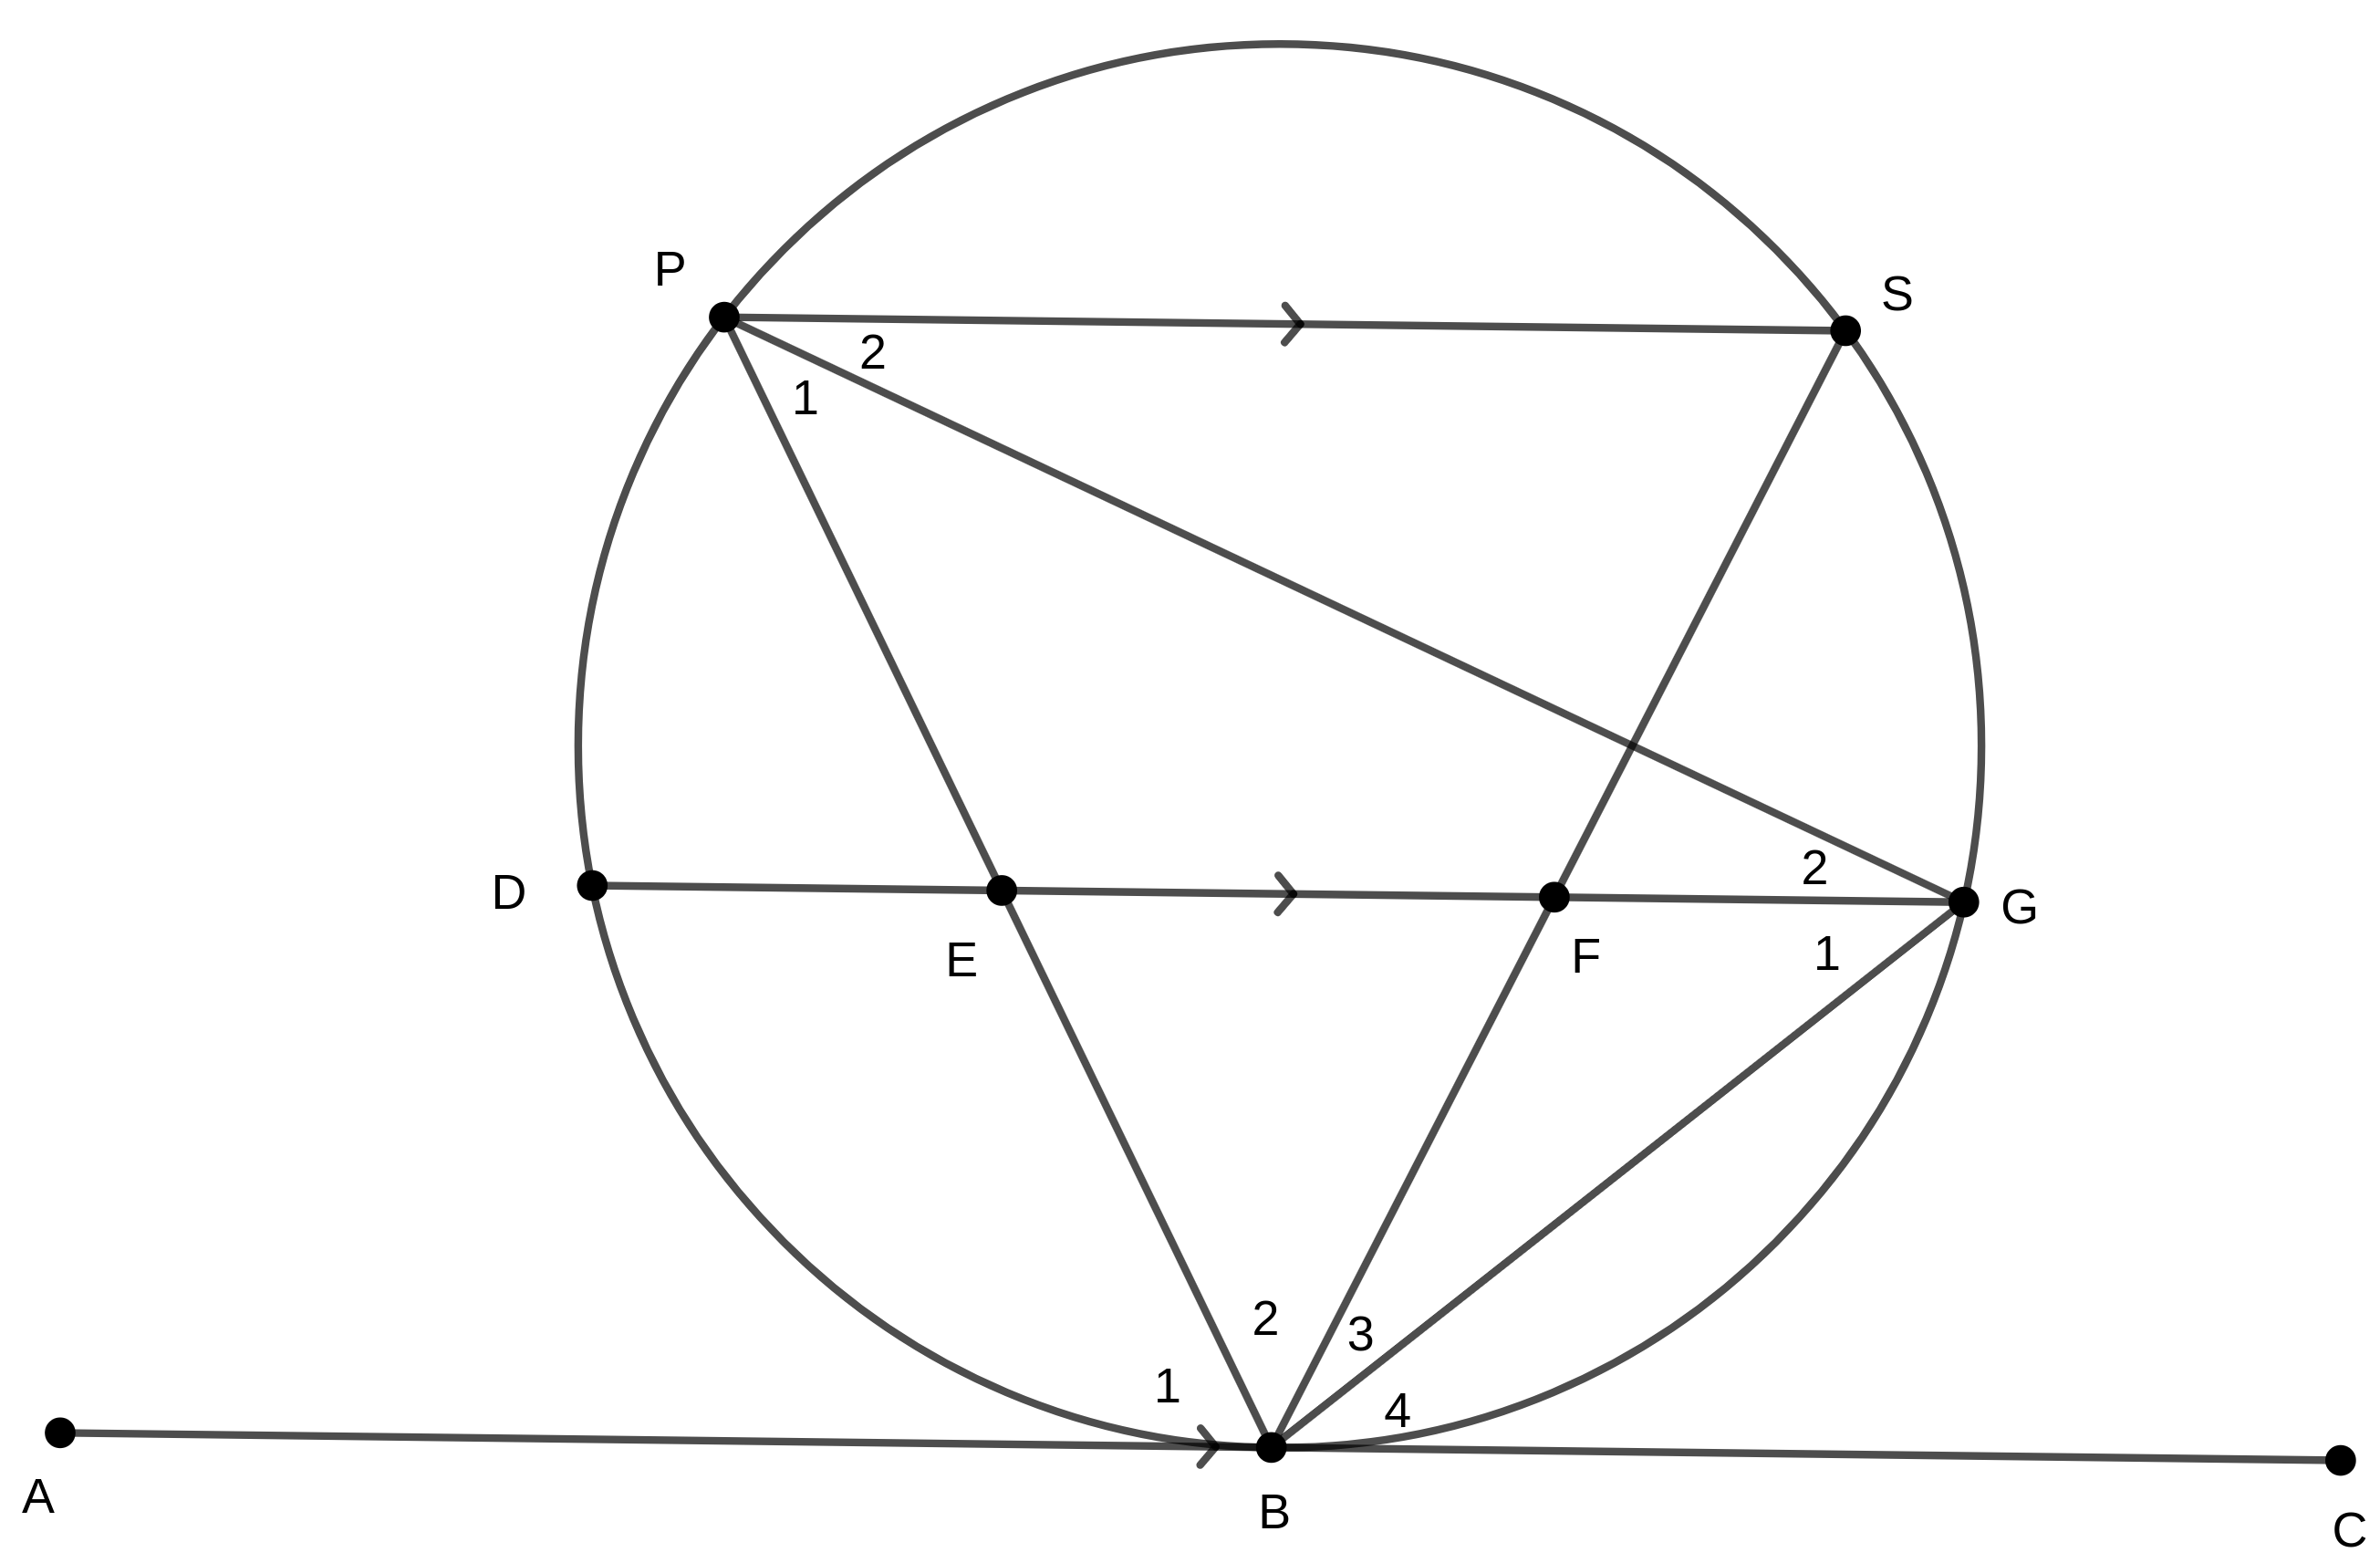
\includegraphics[width = 0.8\linewidth]{test3_geometry1.png}
\end{figure}
  

\vspace{6pt}
\item 
Consider a game wherein two players Emma and Dylan take turns to take between 1 and 7 stones, inclusive, from a pile which starts with 2018 stones. If Emma plays first, does one of the players have a winning strategy, and if so what is it?


\vspace{6pt}
\item Determine all solutions $(x,y)$ of the system of equations
\begin{align*}
  \frac{4}{x} +\frac{5}{y^2} &= 12, \\
  \frac{3}{x} +\frac{7}{y^2} &= 22.
\end{align*}


\item 
Suppose $k$ is a positive integer that does not divide $2008$. Let $[x]$ denote the greatest integer less than or equal to $x$. For example, $[11.75] = 11$ and $[\pi] = 3$. What is the maximum possible value of $k \times \left[\frac{2018}{k}\right]$?


\vspace{6pt}
\item % 
The student lockers at Olympic High are numbered consecutively beginning with locker number 1. The plastic digits used to number the lockers cost $3$ cents per piece. Thus, it costs $3$ cents to number locker $9$ and $6$ cents to number locker $42$. If it costs R206.91 to label all the lockers, how many lockers are there at the school?


\vspace{6pt}
\item 
Consider the function $f(x) = \frac{1}{1-x}$ and its iterates $f^r$ defined as
\begin{align*}
  f^1(x) &= f(x) \\
  f^2(x) &= f(f(x)) \\
  f^3(x) &= f(f(f(x))) \\
  f^4(x) &= f(f(f(f(x)))),
\end{align*}
and so on. Calculate the value of $f^{2018}(2018)$.


\vspace{6pt}
\item % UK IMO 2001 IMO training problem sheet
Given the equation $x^{2018} = y^x$,
\begin{enumerate}
  \item find all pairs $(x,y)$ of solutions with $x$ prime and $y$ a positive integer;
  \item find all pairs $(x,y)$ of positive integers satisfying the equation.
\end{enumerate}

\end{enumerate}


\vfill
\begin{center}
\begin{BVerbatim}
            |\_/|        D\___/\
            (0_0)         (0_o)
           ==(Y)==         (V)
----------(u)---(u)----oOo--U--oOo---
__|_______|_______|_______|_______|___
\end{BVerbatim}
\end{center}

\end{document}
